% !TeX spellcheck = sk_SK
\chapter{Prehľad existujúcich	metód riadenia pre	Dvojkolesové balansujúce roboty}

Balansujúci robot predstavuje z mechanického hľadiska inherentne nestabilnú sústavu, ktorú je pre to, aby bol takýto robot v praxi použiteľný, potrebné stabilizovať pomocou regulátora. V už existujúcich prácach sa stretávame s rôznymi druhmi implementovaných regulátorov a je teda namieste uviesť aspoň niektoré z najčastejšie používaných. V nasledujúcej časti práce sa teda budeme zaoberať  stručným popisom v praxi používaných regulátorov a uvedieme ako sme sa rozhodovali pri výbere regulátora my.

Vo všeobecnosti môžeme ako regulátor označiť každé zariadenie, ktoré v systéme zabezpečuje udržiavanie určitých fyzikálnych veličín na stanovených úrovniach. V priebehu regulácie sa pravidelne zisťuje skutočný stav objektu a porovnáva sa s požadovaným.  Regulátor následne upravuje stav systému tak, aby bol dosiahnutý požadovaný cieľ.

Jedným zo základných spôsobov rozdelenie regulátorov je na lineárne a nelineárne regulátory. Lineárne regulátory sú určené na riadenie sústav, ktorých prenosové funkcie sa vyznačujú tým, že pre ne platí princíp homogenity a superpozície. Pokiaľ chceme použiť takýto regulátor na riadenie nelineárnej sústavy, t.j. sústavy, pre ktorú neplatí princíp homogenity alebo superpozície, bude takýto regulátor pracovať korektne len ak sústava zotrvá v okolí bodu, kde je možné nájsť jej lineárnu aproximáciu. Tento proces sa nazýva linearizácia. 

Pri nelineárnych regulátoroch táto potreba linearizácie odpadá, keďže regulátory tohto typu dokážu pracovať aj s nelineárnymi sústavami. Nevýhodou práce s nelineárnymi sústavami je ale vyššia náročnosť riešenia nelineárnych diferenčných rovníc. Práve kvôli  tomuto problému existuje v praxi tendencia radšej hľadať spôsoby ako čo najpresnejšie reprezentovať nelineárne systémy lineárnymi diferenčnými rovnicami a následne použiť na ich riadenie lineárny regulátor. Je ale nutné ešte podotknúť, že reálne sa pri zohľadnení všetkých vonkajších vplyvov každá sústava javí ako nelineárna. 

Štúdiom prác, ktoré už boli napísané na tému riadenia dvojkolesového balansujúceho robota sme zistili, že medzi regulátory, ktoré sú najčastejšie pre túto úlohu používané patria lineárne regulátory:
\begin{enumerate}
\item \ac{PID} (Proportional Integral Derivative Regulator:PID)
\item \ac{LQR}  (Linear Quadratic Regulator;LQR)
\end{enumerate}

Práve týmito regulátormi sa teda budeme zaoberať v ďalšej podkapitole, no pre úplnosť ešte uvedieme, že vrámci nelineárnych regulátorov sa ako vhodné javia najmä Fuzzy PID a umelé neurónové siete.

\section{Lineárne regulátory}


V tejto časti práce zhrnieme základné poznatky o niektorých vybraných typoch lineárnych regulátoroch. Uvedieme výhodné a nevýhodné vlastnosti jednotlivých regulátorov a v závere zhodnotíme, ktorý sa pre naše potreby javí ako najvhodnejší.

\subsection{PID}


\ac{PID} regulátor je v praxi najčastejšie používaný regulátor, pričom uplatnenie nachádza  pri riadení veličín ako sú napríklad: teplota, tlak, prietok, poloha, atď. Medzi jeho výhodné vlastnosti patrí najmä robustnosť, jednoduchosť implementácie a možnosť manuálneho naladenia bez potreby použitia zložitých výpočtových techník.  Schematické znázornenie jeho zapojenia v ovládanej sústave je na \figurename~\ref{fig:PIDSchematic}

\begin{figure}
\centering
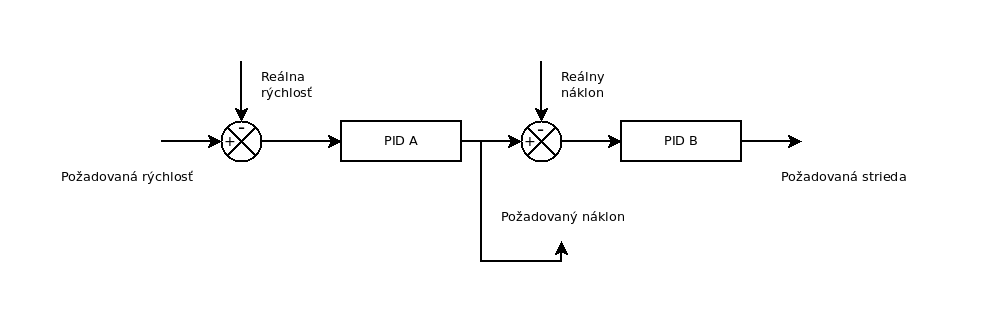
\includegraphics[width=8cm]{PIDSchematic}
\caption{Zapojenie PID}
\label{fig:PIDSchematic}
\end{figure}

Zo schémy je zrejmé, že na vstup privádzame požiadavku na výstup sústavy a od tej následne odčítavame reálne nameranú hodnotu na výstupe (spätná väzba). Takto získavame chybovú veličinu e(t), ktorá vyjadruje nakoľko sa reálna hodnota na výstupe líši od tej požadovanej. Práve s touto chybou ďalej pracuje \ac{PID} regulátor.

Samotný PID regulátor pozostáva z troch častí, ktoré mu zároveň dávajú jeho názov: proporčnej (P), integračnej (I) a derivačnej (D). Každá s týchto častí iným spôsobom reaguje na vstup do PID a proces ladenia tak pozostáva z nastavenia príslušných parametrov (opísaných nižšie) pre jednotlivé tieto časti. Kombináciou rôznych hodnôt parametrov je možné regulátor naladiť tak, aby podľa potrieb používateľa kontroloval výstupnú veličinu. 

\begin{figure}
\centering
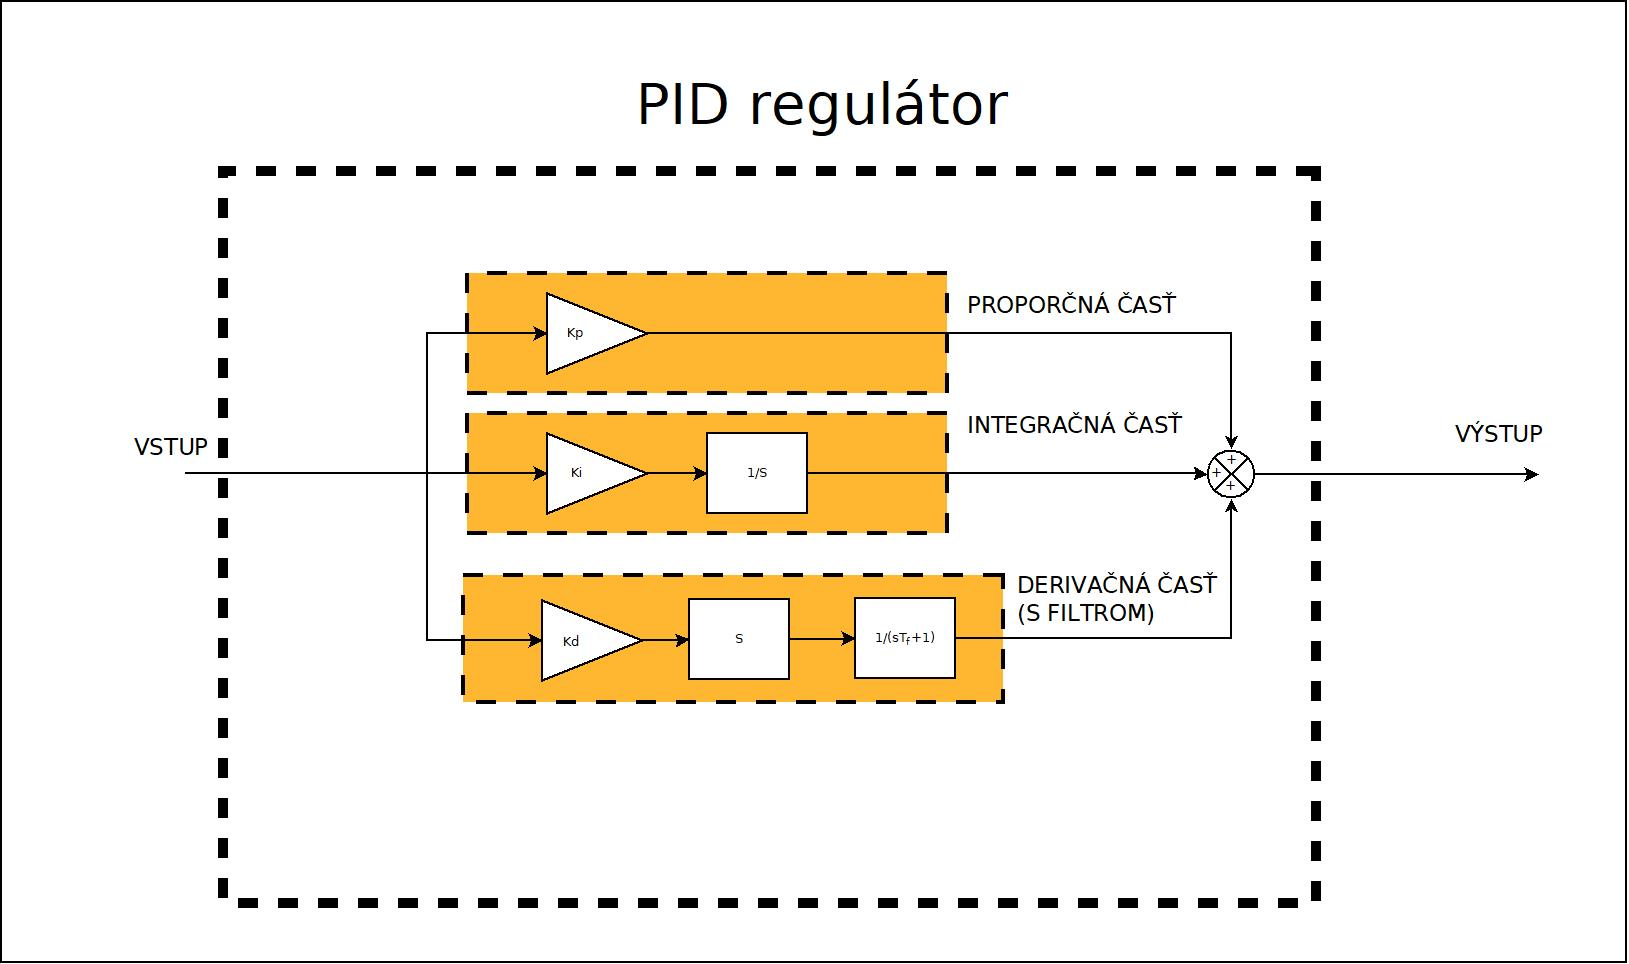
\includegraphics[width=8cm]{PIDComplete}
\caption{Štruktúra PID regulátora}
\label{fig:PIDComplete}
\end{figure}

Vychádzajúc z blokovej schémy na \figurename~\ref{fig:PIDComplete} môžeme podrobne opísať súčasti, z ktorých pozostáva \ac{PID}.

\textbf {Proporčný člen} pozostáva zo zosilňovača, ktorý má na svojom výstupe Kp násobok chyby $e(t)$ . V praxi to teda znamená, že ak je reálny výstup regulovanej sústavy voči požiadavke značne veľký $\rightarrow$ chyba je veľká a záporná, teda proporčný člen reaguje veľkým záporným výstupom. Tento následne zníži veľkosť výstupu a teda aj odchýlku od požadovanej hodnoty. Matematicky je možné vyjadriť výstup proporčného člena ako:

\begin{equation}
u_p (t)= K_p e( t )
\end{equation}

kde up(t) predstavuje výstup a e(t) chybu na vstupe člena v čase t. 

Prípadne je ešte možné použiť vyjadrenie v Laplaceovej rovine vo forme prenosovej funkcie:

\begin{equation}
\dfrac {U_p(s)} {E(s)} = K_p 
\end{equation}
kde $UP(s)$ je výstup a $E(s)$ chyba, vyjadrené v Laplaceovej rovine.

\textbf{Integračný člen} reaguje na súčet chýb, naakumulovaných od spustenia regulátora. Tento súčet je následne vynásobený konštantou $Ki$ a prenesený na výstup integračného bloku. Hlavnou výhodou integračnej časti je, že umožňuje \ac{PID} reagovať aj na veľmi malé konštantné chyby, ktoré by proporčný člen inak nebol schopný korigovať. Aj tá najmenšia chyba voči požiadavke sa totiž procesom integrovania hromadí, až kým je výstup integračného člena dostatočný na jej skorigovanie. 

Matematické vyjadrenie integračného člena je:
\begin{equation}
u_i (t)= K_i \int_0^e \! e( t ) \, \mathrm{d}t 
\end{equation}
kde $u_i(t)$ predstavuje výstup integračného člena v čase $t$. 
Prenosová funkcia je:

\begin{equation}
\dfrac{U_i(s)}{E(s)}  = K_i\dfrac{ 1}{s} 
\end{equation}
kde $U_i (s)$ je výstup vyjadrený v Laplaceovej rovine.

\textbf{Derivačný člen} v základnom zapojení pracuje so zmenou chyby za čas dt (ten sa v ideálnom prípadne limitne blíži k 0). Výhodnou vlastnosťou tohto člena teda je, že pri náhlych zmenách chyby je schopný pružne reagovať veľkou korekciou na výstupe a pri postupnom, pomalom narastaní chyby adekvátne malou korekciou. Zmenou konštanty $Kd$ vieme korigovať silu tejto reakcie na zmenu chyby.

Matematické vyjadrenie derivačného člena je:

\begin{equation}
U_d (t) = K_d\dfrac{ de(t) }{ dt }
\end{equation}
Kde $U_d(t)$ predstavuje výstup integračného člena v čase $t$.
 
Prenosová funkcia je:
\begin{equation}
\dfrac{U_d( s )}{ E(s) } = K_d s
\end{equation}
kde $U_d(s)$ je výstup vyjadrený v Laplaceovej rovine.

Existuje taktiež ale aj iná forma derivačného člena, v ktorej sa počíta so zaradením nízkofrekvenčného filtra určeného konštantou $T_f$ . Použitie tejto formy derivačného člena je obzvlášť výhodné v prípade implementácie derivačného člena na zariadení, ktoré realizuje tento člen v diskrétnej forme (mikropočítač). Pri diskrétnej forme sa totiž ako požiadavka na výstup, tak aj výstup samotný mení skokovo, čo spôsobuje pri absencií filtra silné reakcie derivačného člena, ktoré následne vyvolávajú celkovú nestabilitu  regulovaného systému.  

Filtračný člen má tvar:
\begin{equation}
F_r ( s ) = \dfrac { 1 }{ 1 + T_f s }
\end{equation}
pričom filtračnú konštantu $T_f$  spravidla určujeme podľa vzťahu:
\begin{equation}
T_f =  \dfrac {1} { 2 \pi f_c }
\label{eq:TFconst}
\end{equation}
kde $f_c$ predstavuje najvyššiu frekvenciu signálu, ktorú by ešte filter mal prepustiť. Okrem toh osa ale v praxi používa aj primitívnejšia metóda voľby $T_f$, kedy sa za $T_f$ jednoducho dosadí  celočíselný násobok konštanty $K_d$.

\textbf{Konečná forma PID} sa teda po spočítaní prenosov všetkých členov teda dá zapísať ako:
\begin{equation}
F_{PID} (s) = K_p + K_i \dfrac{1}{s} + K_d s \dfrac{ 1 } { 1 + T_f }
\label{eq:compPID}
\end{equation}

Na samotné naladenie \ac{PID} regulátora je možné použiť viacero metód, medzi inými napríklad:

\begin{itemize}
\item \textbf{Ad–hoc metóda} - veľmi primitívnou, ale pre jednoduché problémy sústavy dostačujúcou metódou je zvolenie $K_p$, $K_i$, $K_d$ parametrov náhodným dosadzovaním a pozorovaním zmien reakcií riadenej sústavy
\item \textbf{Ziegler-Nicholsová metóda} - pozostáva z vyradenia I, D zložiek a nájdenia takej hodnoty Kp, pri ktorej systém dosiahne stav na hranici stability, t.j. stavu, v ktorom sústava osciluje okolo stabilného stavu. V tomto stave odmeriame periódu oscilácií. Následným odčítaním hodnôt$K_p$, $K_i$, $K_d$ z tabuľky \ref{tab:Zieger-Nichols}, prevzatej zo skrípt\cite{SKRIPTA} získame naladený PID.
\item \textbf{Vytvorením modelu sústavy} - po nájdení matematického modelu regulovanej 	sústavy je možné vytvoriť sústavu diferenciálnych rovníc, ktoré popíšu správanie celej sústavy so zaradeným regulátorom. Tento matematický model je možné následne podrobiť analýze pomocou kritérií stability napr. Routh-	Schurovým alebo Hurwitzovým a takto nájsť  $K_p$ , $K_i$ , $K_d$, pre ktoré bude sústava stabilná. Nevýhodou tohoto postupu je ale zvýšená náročnosť procesu ladenia, ale aj nutnosť dostatočne presne poznať štruktúru sústavy na 	vytvorenie jej modelu.  
\end{itemize}

\subsection{LQR}

Pred opisom samotného princípu fungovania LQR, považujeme za potrebné uviesť čitateľa do problematiky reprezentácie systémov v tzv. stavovom priestore, nakoľko regulátor LQR pracuje práve s touto reprezentáciou systému.

Pri reprezentácií časovo invariatnej sústavy, teda sústavy, ktorej vlastnosti sa časom nemenia, v stavovom priestore pracujeme vo všeobecnosti z výrazmi tvaru:

\begin{equation}
\dot {\textbf{x}}(t) = Ax(t) + Bu(t) \linebreak
\textbf {y}(t) = Cx(t) + Dy(t)  
\end{equation}
\newpage
\begin{figure}
\centering
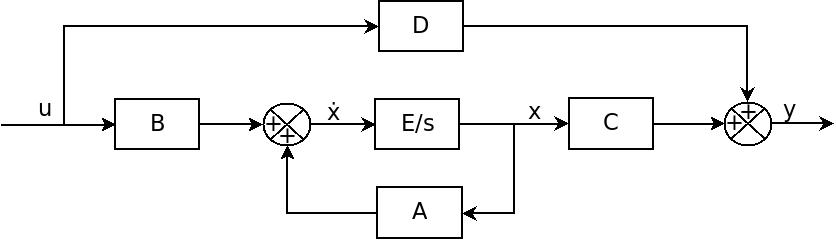
\includegraphics[width=9cm]{stavovyPriestorDiagram}
\caption{Stavový priestor - diagram}
\label{fig:stavovyPriestorDiagram}
\end{figure}

Pri takomto značení:\newline
$A$ = stavová matica systému [n x n]\newline
$B$ = vstupná matica [n x r]\newline
$C$ = výstupná matica [m x n]\newline
$D$ = matica opisujúca priamy prenos na výstup systému [m x r]\newline
$x(t)$ = stavový vektor [n x 1]\newline
$y(t)$ = výstupný vektor [m x 1]\newline
$u(t)$ = vstupný vektor [r x 1]\newline
$\dot{x}(t)$ = prvá derivácia stavového vektora [n x 1]
pričom platí, že m, n, r $\subset$ N. 

Výhody takejto reprezentácie sústav sa prejavia hlavne pri MIMO sústavách (sústavách ktoré majú viacero vstupov a výstupov). S využitím maticovej a vektorovej reprezentácie je možné aj veľmi komplexné systémy vyjadriť len pomocou týchto dvoch rovníc. Maticová reprezentácia je naviac ešte aj veľmi vhodná pre spracovanie s využitím softvérových nástrojov ako napr. Matlab.

Proces samotného vyjadrenia stavovej reprezentácie zo systému diferenciálnych rovníc je mimo rozsah tejto práce, čitateľ sa však s ním môže oboznámiť v ...

\todo[inline]{doplniť odkazy}

Po nájdení reprezentácie v stavovom priestore a overení, že daný systém je kontrolovateľný, môžeme z matice A vyjadriť póly stavovej matice sústavy. To je možné napr. výpočtom z rovnice:

\begin{equation}
\mid pE - A \mid = 0 
\end{equation}

Kde E je jednotková matica a p vektor pólov matice A.

	Pripomenieme, že pre stabilné systémy platí, že všetky reálne časti ich pólov sú záporné. Tento poznatok je možné účinne využiť v prípade nestabilných systémov a zaradiť do sústavy vhodne zvolený regulačný vektor K, ktorý nám zavedením spätnej väzby do sústavy umožní zmeniť pôvodné póly na ľubovoľné, nami zvolené, stabilné $(Re{pi}<0)$ póly. 

Reprezentácia takejto sústavy v stavovom priestore bude mať následne tvar:
\begin{equation}
u( t ) = -Kx
\label{eq:ut}
\end{equation}
\begin{equation}
\dot{\textbf{x}}(t) = Ax(t) + B(-Kx(t))
\label{eq:xDot}
\end{equation}

\begin{figure}
\centering
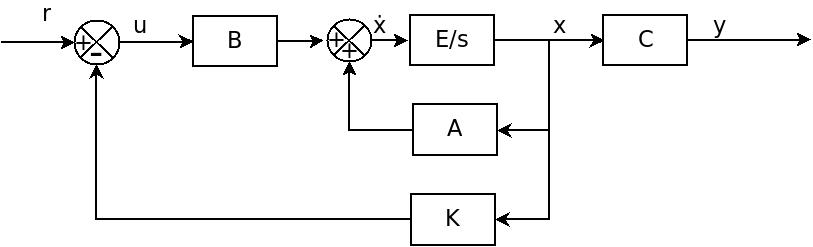
\includegraphics[width=9cm]{stavovyPriestorSV}
\caption{Stavový priestor - spätná väzba}
\label{fig:stavovyPriestorSV}
\end{figure}

Čitateľ si môže všimnúť, že na \figurename~\ref{fig:stavovyPriestorSV} už nevystupuje v schéme matica D, ktorú v danom prípade uvažujeme ako nulovú – veličina na vstupe nie je teda privádzaná priamo na výstup. Členom r v schéme na \figurename~\ref{fig:stavovyPriestorSV} rozumieme referenciu, ktorej zmenou vieme upraviť požiadavku na výstup systému.

Vyššie sme spomínali, že vektor K je možné zvoliť tak aby boli dosiahnuté požadované póly, problémom ale je určiť aké póly sú pre danú sústavu ideálne. Pri zvolení príliš negatívnych pólov bude regulátor natoľko agresívny, že ho nebude možné v praxi realizovať a naopak, pokiaľ nebudú póly dostatočne záporné, bude regulácia trvať pridlho na to aby bola praktická.  Práve tu prichádza ako riešenie do úvahy regulátor LQR, ktorý je využitím kvadratickej „cenovej“ funkcie schopný prideliť každej sledovanej veličine na výstupe „váhu“. Táto váha určí nakoľko budú pre regulátor dôležité zmeny jednotlivých veličín. LQR následne zvolí K také, aby regulátor pracoval podľa požiadaviek.

Ako vyplýva z názvu regulátora, pre svoju činnosť využíva princíp minimalizácie cenovej funkcie J, ktorá je pre spojitý a konečný časový úsek definovaná ako:

\begin{equation}
J = \dfrac {1} {2} x^T (T)P_1 x(T)  + \dfrac {1} {2} \int_0^T \! ( x^T Qx + u^T Ru) \, \mathrm{d}t 
\label{eq:cenovaFunkcia}
\end{equation}

kde $Q \geq 0$; $R > 0$; $P1 \geq 0$ sú symetrické, kladné matice. $Q$,$ R$ predstavujú váhy, ktoré sú priradené sledovaným veličinám.
Riešením rovnice \figurename~\ref{eq:cenovaFunkcia} je $P(t)$, nájdené vyriešením tzv. aritmetickej Riccatiho rovnice :

\begin{equation}
- \dot {P} = PA + A^T P - PBR^{-1} B^T P + Q;	\newline
P( T ) = P_1
\label{eq:riccatiEq}
\end{equation}

Následkom rovnice \figurename~\ref{eq:riccatiEq} je po spätnom chode a vyriešení pre $K$ možné vyjadriť $u(t)$ z rovnice \figurename~\ref{eq:ut} ako:
\begin{equation}
u( t ) = -R^{-1} B^T P( t )x
\end{equation}

Keďže riešenie týchto rovníc je do značnej miery komplikované a jednoznačne mimo rozsah tejto práce uvedieme len, že pri použití nastroja Matlab je možné nájsť K veľmi jednoducho a to použitím funkcie: K = lqr(A, B, Q, R).

Pred implementáciou LQR je ale ešte potrebné adresovať otázku voľby R, Q matíc. Predpokladajme matematický model balansujúceho robota v stavovom priestore vyjadrený dosadením do rovnice \figurename~\ref{eq:xDot} ako:
\begin{equation}
\dot {\textbf {x}} = (A - BK) \begin{bmatrix}
d \\
\dot{d} \\
\theta \\
\dot{\theta} 
\end{bmatrix}
\end{equation}
kde: 

\quad $d$ = poloha základne robota 

\quad $\dot{d}$ rýchlosť  základne robota 

\quad $\theta$ = uhol natočenia šasi robota 

\quad $\dot{\theta}$ = uhlová rýchlosť robota

Ďalej uvažujeme Q také, že:
\begin{equation}
Q = \begin{bmatrix}
w_1 & 0 & 0 & 0 \\
0 & w_2 & 0 & 0 \\
0 & 0 & w_3 & 0 \\
0 & 0 & 0 & w_4
\end{bmatrix}
\end{equation}
\newline
Predpokladajme, že maximálne dovolené odchýlky od požadovanej hodnoty sú:
\begin{itemize}
\item $0,005 m $pre polohu základne → $w_1$ = $(0,005)^{-2}$
\item $0,0005 m.s^-1$ pre rýchlosť základne → $w_2$ = $(0,0005)^{-2}$
\item $0,02 rad$ pre uhlovú odchýlku šasi → $w_3$ = $(0,02)^{-2}$
\item $0,0001 rad.s^{-1}$ pre uhlovú rýchlosť šasi → $w_4$ = $(0,0001)^{-2}$
\end{itemize}

Po určení Q by sme podobným spôsobom postupovali aj pre R až kým by sme našli hodnoty, ktoré pre sústavu fungujú uspokojivo. 

\section{Zhrnutie a výber regulátora}
Medzi značné výhody PID regulátora patrí jeho jednoduchá implementácia a nízka náročnosť na výpočtový výkon realizačného hardvéru. Ladenie je možné ako exaktnými, matematickými metódami tak aj metódami založenými na empiricky zozbieraných dátach. Nevýhodou PID je ale,  že jeho využitie je obmedzené na SISO systémy, t.j. systémy s jednou vstupnou a jednou výstupnou veličinou – čo napríklad v našom prípade nezaručí stabilizáciu polohy aj riadenie robota súčastne. Tento nedostatok je ale možné prekonať použitím viacerých vhodne kombinovaných PID regulátorov, čo však zvyšuje náročnosť ich správneho naladenia.

Hlavnou výhodou využitia LQR na reguláciu sústavy je, možnosť riadiť jediným regulátorom všetky nami sledované výstupné veličiny, čim je možné dosiahnuť veľmi komplexné riadenie robota. Pri návrhu regulátora je taktiež možné zvoliť, ktoré sledované veličiny sú pre nás najdôležitejšie. Cenou za takúto presnosť riadenia je ale výrazne vyššia náročnosť výpočtov pri ladení regulátora ako aj nutnosť pracovať s matematickým modelom sústavy. Komplikovanejšie výpočty taktiež spôsobia, že v porovnaní s PID bude dĺžka trvania riadiacej slučky pri použití totožného hárdveru dlhšia čo môže viesť k zhoršeniu vlastností robota.

Po zohľadnení vlastností oboch regulátorov sme sa rozhodli pre použitie PID regulátora. Napriek niektorým jeho nevýhodným vlastnostiam bola jednoduchosť jeho implementácie rozhodujúcim faktorom pri našej voľbe. Viacero prác už demonštrovalo uspokojivé výsledky pri použití PID na riadenie balansujúceho robota a teda vieme, že ide o regulátor dostačujúci na naše účely a na rozdiel od LQR má autor s jeho používaním predošlé skúsenosti. 

Kvôli neschopnosti PID riadiť viacero výstupov zároveň budeme pri našej realizácií pracovať s viacerými PID regulátormi zaradenými do kaskády. V takomto zapojení sa zvyčajne uvažuje používa rozdielna dĺžka riadiacich slučiek - teda  rozdielne dt pre jednotlivé PID. Viac sa danou problematikou budeme zaoberať priamo v kapitole venovanej našej implementácií regulátora.